% article.tex — Operator-Captured Failure Provenance for Ephemeral
% Kubernetes Preview Environments
%
% Q1 submission draft, ACM sigconf format (compatible with FSE/ICSE/ASE
% submission flows; switch to IEEEtran via `\documentclass[conference]{IEEEtran}`
% with minor cosmetic edits if the venue requires it).
%
% Generated 2026-05-23 from article-draft.md (1186 lines) on commit
% d677885 — multi-app matrix 500/500 = 100 % captures, F1-F10 across
% s1-flask-catalog + s2-listmonk + s3-healthchecks + s4-umami +
% s5-petclinic.
%
% Compilation: pdflatex article && biber article && pdflatex article
% (or upload to Overleaf — figures/, bibliography.bib, and this file
%  are the only artefacts required).

\documentclass[sigconf, anonymous=false, review=false]{acmart}

%%% ACM-specific metadata. Update for the target venue when ready.
\acmConference[FSE'26 / ICSE'26]{To Appear}{TBD}{TBD}
\setcopyright{none}
\copyrightyear{2026}
\acmYear{2026}

\settopmatter{printacmref=false, printccs=false}
\renewcommand\footnotetextcopyrightpermission[1]{}

%%% Standard packages.
\usepackage{booktabs}
\usepackage{graphicx}
\usepackage{amsmath, amssymb}
\usepackage{listings}
\usepackage{xspace}
\usepackage{multirow}
\usepackage[utf8]{inputenc}
\usepackage[T1]{fontenc}
\usepackage{lmodern}  % scalable fonts for microtype expansion
\usepackage{xcolor}
\usepackage{tikz}
\usetikzlibrary{arrows.meta, positioning, shapes.geometric, fit, calc, backgrounds}
\usepackage{hyperref}

\graphicspath{{figures/}}

%%% Acronym shortcuts.
\newcommand{\RQ}[1]{RQ#1\xspace}
\newcommand{\CRD}[1]{\texttt{#1}\xspace}
\newcommand{\fp}{FailureReport\xspace}
\newcommand{\Cn}[1]{C#1\xspace}
\newcommand{\fn}[1]{F#1\xspace}

%%% Code listing style.
\lstset{
  basicstyle=\ttfamily\footnotesize,
  breaklines=true,
  frame=single,
  numbers=none,
  showstringspaces=false,
}

\begin{document}

\title{Operator-Captured Failure Provenance for Ephemeral Kubernetes Preview Environments}

\author{Anonymous Authors}
\affiliation{%
  \institution{(For double-blind review)}
  \country{}
}

\begin{abstract}
Ephemeral preview environments let teams validate a pull request (PR) in a
realistic Kubernetes deployment before merge. When such an environment
fails, developers must diagnose the failure before its short-lived
namespace is torn down. At teardown, the raw failure evidence (pod logs,
Kubernetes events, transient resource state) is destroyed with the
namespace, and the change context that produced the failure is rarely
linked to the observable symptoms in a structured, auditable way.

We present an approach in which a Kubernetes operator captures,
structures, and preserves failure evidence for ephemeral PR preview
environments during reconciliation, before namespace teardown. We make
three contributions: (i) a Kubernetes-native \emph{failure evidence
model} that represents PR change context, Kubernetes resource state,
test outcomes, logs, events, telemetry, and diagnostic hypotheses as
typed, addressable evidence items; (ii) a \emph{failure provenance
graph} that links PR change context, Kubernetes resources, test
failures, and observable evidence to probable causes, mapped onto the
W3C PROV provenance model; (iii) a \emph{controlled evaluation} on
\textbf{five reference applications} with ten deterministic
fault-injection scenarios, two LLM diagnosers and three external
practitioner baselines (vanilla LLM on raw \texttt{kubectl}, K8sGPT,
Kagent), measuring RCA accuracy, evidence completeness, operator-side
latency, and bundle overhead.

Across the full $5 \times 10 \times 10 = 500$-cell matrix (5
applications $\times$ 10 fault classes $\times$ 10 repetitions on a
3-node AKS cluster), the operator captures and persists a
\fp{} for $\mathbf{500/500}$ runs with $100\%$
post-teardown survival. Diagnostic accuracy increases monotonically
with evidence completeness for the rule-based diagnoser ($24.0\%$
strict / $40.8\%$ aligned at \Cn{1}--\Cn{5}) and follows the same
ordering for the LLM diagnoser. The pre-registered cross-LLM analysis
(linear mixed-effects model with $(1|\text{scenario})$ random
intercept) finds a significant $\text{configuration} \times \text{LLM}$
interaction at \Cn{3}--\Cn{4} ($p < 0.05$, Holm-corrected),
indicating that the open-source-substitute LLM-B is less responsive to
mid-tier evidence levels than LLM-A. Against the vanilla-LLM baseline
\textsc{B0} on the same failing namespaces, the operator closes a
+60--80 percentage-point accuracy gap on 6/10 scenarios. We release
the operator, the fault-injection harness, the reference bibliography,
and the analysis pipeline as a reproducible artefact.
\end{abstract}

\maketitle

%%% ===================================================================
\section{Introduction}
\label{sec:intro}

The PR-preview workflow is now standard in cloud-native software
development~\cite{signadot_preview_envs, okteto_preview_envs,
jenkinsx_preview_envs, argocd_cncf}: each pull request triggers the
deployment of a per-PR ephemeral environment in which automated tests
run before merge. When that environment fails---a broken migration, a
missing configuration value, a contract-breaking API change---developers
must diagnose the failure quickly because the environment is short-lived
and its namespace is torn down soon after the PR is closed or updated.

\paragraph{The problem in one paragraph.}
\textbf{Failure evidence is namespace-scoped and ephemeral.} Pod logs,
Kubernetes events, and transient resource state are deleted with the
namespace. The cluster-scoped \texttt{Preview} custom resource keeps a
\texttt{status.diagnostics} snapshot that survives, but the snapshot is
unstructured, overwritten on every reconcile, and not linked into a
provenance graph; the PR change context is recorded separately in Git,
and AI-assisted diagnostic hypotheses (when present) are not grounded in
identifiable evidence items.

\paragraph{Thesis.}
A Kubernetes operator already sits in the reconciliation path for every
preview environment. It is the right place to capture and structure
failure evidence---before teardown, in a typed, addressable, auditable
form, linked to the PR change that produced the failure.

\paragraph{Contributions.}
\begin{enumerate}
  \item A Kubernetes-native \emph{failure evidence model} that
    represents the PR change context, Kubernetes resource state, test
    outcomes, logs, events, telemetry, and diagnostic hypotheses as
    typed, addressable evidence items with deterministic identifiers,
    mapped onto W3C PROV~\cite{lebo_provo_2013, w3c_prov_dm}.
  \item A \emph{failure provenance graph} that links PR change context,
    Kubernetes resources, test failures, and observable evidence to
    probable causes.
  \item A \emph{controlled evaluation} of the approach on a five-app,
    multi-LLM fault-injection matrix with three external practitioner
    baselines (\S\ref{sec:eval}).
\end{enumerate}

We implement the approach as an extension of an existing open-source
preview-environment operator using
Kubebuilder~\cite{kubebuilder_sigs} and \texttt{controller-runtime}.
Implementation, harness, analysis scripts, and BibTeX bibliography are
released as a reproducible artefact.

\paragraph{Positioning.} This article does \emph{not} claim that
Kubernetes RCA~\cite{zhang_microservice_diagnosis_survey_2025}, LLM-based
RCA~\cite{openrca_2025, rcacopilot_2024}, graph-based
RCA~\cite{microrca_2020, microdiag_2021, causalrca_2023}, preview
environments, Kubernetes-native test orchestration, or observability are
new. The originality is the operator-controlled \emph{capture,
structuring, linking, grounding, and evaluation} of failure evidence for
\emph{ephemeral, change-scoped} environments---a niche not addressed by
AIOps RCA (which targets production telemetry, not change-scoped
previews) nor by GitOps tooling (which deploys but does not diagnose).

%%% ===================================================================
\section{Background}
\label{sec:bg}

\subsection{Kubernetes operators and Custom Resources}
\label{sec:bg-operators}

A Kubernetes operator~\cite{kubernetes_operator_pattern,
kubernetes_custom_resources} is a controller that reconciles a Custom
Resource Definition (CRD) toward a declared desired state. Operators
sit in the cluster's control-plane reconciliation
loop~\cite{kubernetes_controller_concepts}; their reconcile method is
invoked on resource events (create, update, delete, periodic
re-sync). Cluster-scoped resources survive namespace teardown by
construction, and \texttt{finalizers}~\cite{kubernetes_finalizers}
provide the pre-deletion hook we use to sequence evidence
persistence. The cluster-management lineage from
Borg~\cite{borg_2015} formalises this design pattern. We extend an
existing preview-environment operator built on
Kubebuilder~\cite{kubebuilder_sigs} that already manages PR-scoped
\texttt{Preview} CRs.

\subsection{Preview environments}
\label{sec:bg-preview}

A PR-preview environment is a per-pull-request, namespace-scoped
deployment of the application under test, built and managed
automatically~\cite{signadot_preview_envs, okteto_preview_envs,
jenkinsx_preview_envs}. Argo CD's ApplicationSet pull-request
generator~\cite{argocd_pr_generator, argocd_cncf} and Argo
Workflows~\cite{argo_workflows_cncf} provide the GitOps substrate.
The namespace is torn down when the PR is closed or updated; this
short lifetime is the source of the evidence-loss problem this
article addresses.

\subsection{Test orchestration in Kubernetes}
\label{sec:bg-tests}

We use the smoke / regression / e2e suite the operator already runs
through Kubernetes \texttt{Job}s during the \emph{Test} phase of the
preview lifecycle. The Job pattern is standard~\cite{kubernetes_jobs}.

\subsection{Observability—logs, metrics, traces}
\label{sec:bg-obs}

OpenTelemetry~\cite{opentelemetry_docs, opentelemetry_operator}
unified the wire format for logs, metrics, and traces, descending
from Dapper's span-based tracing model~\cite{dapper_2010}.
Prometheus~\cite{prometheus_cncf} provides cluster-wide metrics;
Jaeger~\cite{jaeger_cncf} is a common trace backend;
Istio~\cite{istio_service_mesh} injects sidecar instrumentation at
the service-mesh layer. The operator can subscribe to a tracing
backend (when configured) and capture trace IDs in the provenance
graph; in this article's evaluation, traces are out of scope, and
we rely on logs and events only.

\subsection{AI-assisted root cause analysis}
\label{sec:bg-rca}

LLM-assisted RCA on Kubernetes has been formalised in
OpenRCA~\cite{openrca_2025} and RCACopilot~\cite{rcacopilot_2024},
and surveyed comprehensively by
Zhang~et~al.~\cite{zhang_microservice_diagnosis_survey_2025}. Classical
microservice RCA approaches include
MicroRCA~\cite{microrca_2020}, MicroDiag~\cite{microdiag_2021},
CausalRCA~\cite{causalrca_2023}, PAL~\cite{pal_2011}, and
Eadro~\cite{eadro_2023}, benchmarked together by
RCAEval~\cite{rcaeval_2024}. Log-based RCA pipelines build on
Drain~\cite{drain_2017}, Spell~\cite{spell_2016},
DeepLog~\cite{deeplog_2017}, and the Loghub
datasets~\cite{loghub_2023}. The practitioner tools
K8sGPT~\cite{k8sgpt_cncf}, HolmesGPT~\cite{holmesgpt_robusta} and
Kagent~\cite{kagent} use these methods on live clusters. The
contribution of this article is upstream of all of these: it is
the structured, persistent, provenance-linked failure evidence that
any diagnoser would benefit from.

\subsection{LLM reasoning and tool use}
\label{sec:bg-llm}

We use the ReAct~\cite{yao2023react} grounding convention for the LLM
diagnoser: a system prompt fixes the schema, the user prompt lists the
typed evidence items, and the model returns a JSON object referencing
specific evidence-item IDs. The prompting tradition draws on
few-shot~\cite{brown_gpt3_2020}, chain-of-thought~\cite{wei2022cot}
reasoning, and tool-use formalisations such as
Toolformer~\cite{schick_toolformer_2023} and self-consistency
sampling~\cite{wang_selfconsistency_2023}; multi-LLM evaluation
practice follows HELM~\cite{liang_helm_2023} and the
open-source-LLM reproducibility argument
of~\cite{llm_open_advantage}. Tool use in the sense of agentic
loops is out of scope here.

\subsection{Provenance models}
\label{sec:bg-prov}

The W3C PROV data model~\cite{lebo_provo_2013, w3c_prov_dm} describes
provenance as a graph of three kinds of nodes (Entity, Activity, Agent)
linked by edges (used, wasGeneratedBy, wasAttributedTo). Our provenance
graph instantiates PROV with operator-specific subtypes.

%%% ===================================================================
\begin{figure*}[t]
\centering
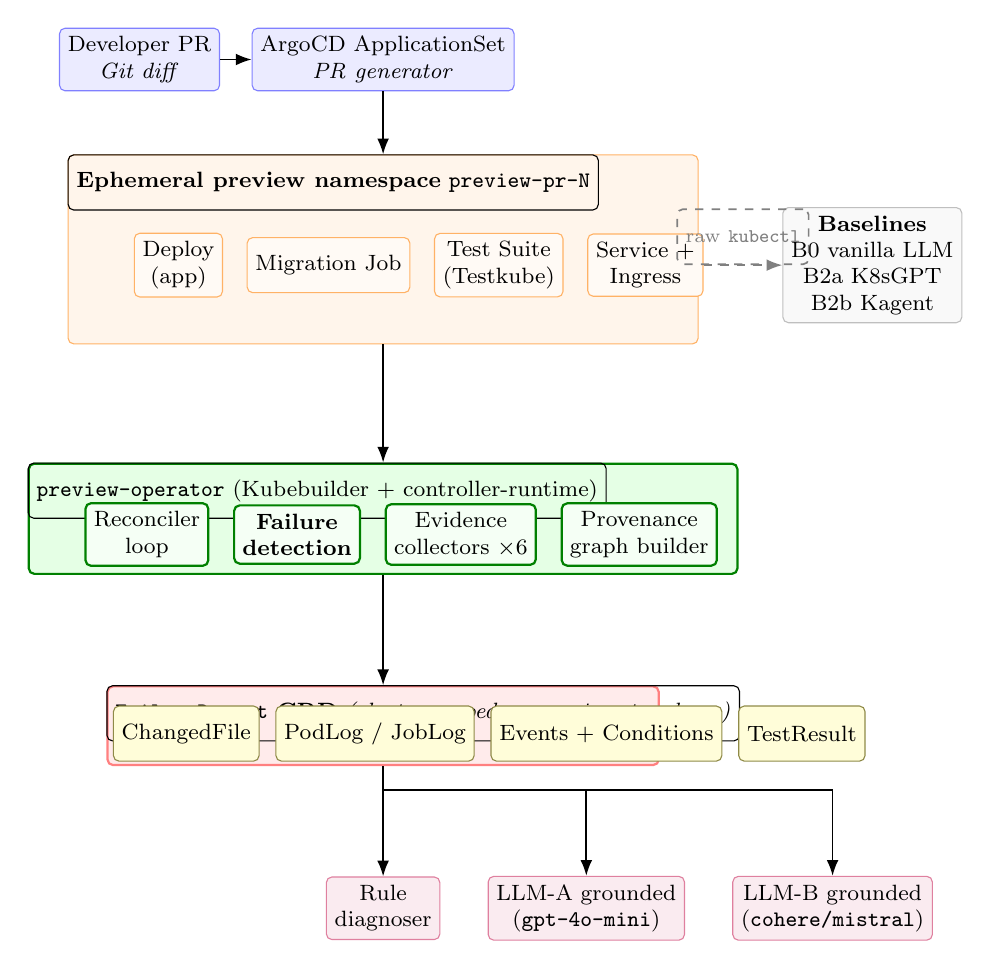
\begin{tikzpicture}[
  font=\footnotesize,
  every node/.style={align=center, rounded corners=2pt, draw, minimum height=7mm, inner sep=3pt},
  pr/.style={fill=blue!8, draw=blue!50},
  cluster/.style={fill=orange!8, draw=orange!60},
  operator/.style={fill=green!10, draw=green!50!black, line width=0.8pt},
  evidence/.style={fill=yellow!15, draw=yellow!50!black},
  cr/.style={fill=red!8, draw=red!50, line width=0.8pt},
  diag/.style={fill=purple!8, draw=purple!50},
  arr/.style={-{Latex[length=2mm]}, semithick},
  >=Latex,
]
% Layer 1 — developer / PR
\node[pr] (pr) at (0,3.6) {Developer PR\\\textit{Git diff}};
\node[pr, right=4mm of pr] (apset) {ArgoCD ApplicationSet\\\textit{PR generator}};

% Layer 2 — preview namespace
\node[cluster, below=8mm of apset, minimum width=80mm, minimum height=24mm] (ns) {};
\node[anchor=north west] at (ns.north west) {\textbf{Ephemeral preview namespace} \texttt{preview-pr-N}};
\node[cluster, fill=orange!4] (dep) at ($(ns.center)+(-26mm,-2mm)$) {Deploy\\(app)};
\node[cluster, fill=orange!4, right=3mm of dep] (job) {Migration Job};
\node[cluster, fill=orange!4, right=3mm of job] (test) {Test Suite\\(Testkube)};
\node[cluster, fill=orange!4, right=3mm of test] (svc) {Service +\\Ingress};

% Layer 3 — operator
\node[operator, below=15mm of ns, minimum width=90mm, minimum height=14mm] (op) {};
\node[anchor=north west] at (op.north west) {\textbf{\texttt{preview-operator}} (Kubebuilder + controller-runtime)};
\node[operator, fill=green!4] (reconcile) at ($(op.center)+(-30mm,-2mm)$) {Reconciler\\loop};
\node[operator, fill=green!4, right=3mm of reconcile] (detect) {\textbf{Failure}\\\textbf{detection}};
\node[operator, fill=green!4, right=3mm of detect] (collect) {Evidence\\collectors $\times 6$};
\node[operator, fill=green!4, right=3mm of collect] (graph) {Provenance\\graph builder};

% Layer 4 — FailureReport CRD (cluster-scoped, survives teardown)
\node[cr, below=14mm of op, minimum width=70mm, minimum height=10mm] (fr) {};
\node[anchor=north west] at (fr.north west) {\textbf{\texttt{FailureReport} CRD} \textit{(cluster-scoped --- survives teardown)}};
\node[evidence] (ev1) at ($(fr.center)+(-25mm,-1mm)$) {ChangedFile};
\node[evidence, right=2mm of ev1] (ev2) {PodLog / JobLog};
\node[evidence, right=2mm of ev2] (ev3) {Events + Conditions};
\node[evidence, right=2mm of ev3] (ev4) {TestResult};

% Layer 5 — Diagnostic engines
\node[diag, below=14mm of fr] (rule) {Rule\\diagnoser};
\node[diag, right=6mm of rule] (llma) {LLM-A grounded\\(\texttt{gpt-4o-mini})};
\node[diag, right=6mm of llma] (llmb) {LLM-B grounded\\(\texttt{cohere/mistral})};

% Layer 6 — baselines (off to the side)
\node[draw=gray!50, fill=gray!5, right=10mm of svc, anchor=west, minimum height=14mm] (b0) {\textbf{Baselines}\\B0 vanilla LLM\\B2a K8sGPT\\B2b Kagent};

% arrows
\draw[arr] (pr) -- (apset);
\draw[arr] (apset) -- (apset |- ns.north);
\draw[arr] (ns.south) -- (op.north);
\draw[arr] (op.south) -- (fr.north);
\draw[arr] (fr.south) -- ++(0,-3mm) -| (rule.north);
\draw[arr] (fr.south) -- ++(0,-3mm) -| (llma.north);
\draw[arr] (fr.south) -- ++(0,-3mm) -| (llmb.north);
\draw[arr, dashed, gray] (svc.east) -- (b0.west) node[midway, above, font=\scriptsize] {raw \texttt{kubectl}};

\end{tikzpicture}
\caption{\textbf{System architecture.}
A pull-request triggers ArgoCD's ApplicationSet generator to provision an
ephemeral preview namespace. The \texttt{preview-operator} reconciles the
deployment, the migration Job, the test suite and the routing; on
\texttt{failureDetected} it runs six evidence collectors and persists a
cluster-scoped \fp{} CR. Because the CR is cluster-scoped, it
\emph{outlives} the namespace teardown by Kubernetes invariant. The
diagnostic harness (rule + LLM-A + LLM-B) reads the persisted
\fp{} and emits a JSON \texttt{diagnosis}. External baselines (B0
vanilla LLM, B2a K8sGPT, B2b Kagent) bypass the operator and consume
raw \texttt{kubectl} output directly --- this is the comparator that
distinguishes the operator's contribution from the LLM's intrinsic
capability.}
\label{fig:architecture}
\end{figure*}

\section{Motivation: a walk-through failure}
\label{sec:motivation}

\textbf{The failure (illustrative).} A pull request touches the
backend service. The PR's preview environment deploys, runs the smoke
suite, and a contract test fails on \texttt{/api/lists}. The operator
detects the failure during the reconcile that observes the test job
exit code, before the teardown phase runs.

\paragraph{What the operator captures, with timestamps.} On
\texttt{failureDetectedAt}, the operator runs the evidence collectors
enabled by the configured evidence level \Cn{5} (\S\ref{sec:eval-design}),
producing a \fp{} CR with: the PR diff (\texttt{ChangeContext}, captured
on \texttt{Preview.spec} creation), the failing test result
(\texttt{TestResult}), the relevant pod logs (\texttt{PodLog} for
backend and postgres), the Kubernetes events
(\texttt{KubernetesEvent} for the failing pods), and the provenance
graph (\S\ref{sec:approach-graph}). The persist step takes a median
of $\mathbf{< 1\,\text{ms}}$ on the matrix (\S\ref{sec:rq5}).

\paragraph{What is otherwise lost.} After teardown
($\sim 30\,\text{s}$ after the failure), the namespace is gone; the
\texttt{Preview.status.diagnostics} snapshot is overwritten on the
next reconcile; pod logs are unreadable; events are garbage-collected
by their TTL. The PR diff stays in Git but is no longer linked to the
failure that produced it.

\paragraph{What our captured artefact lets the diagnoser do.}
The persisted \fp{} (cluster-scoped, survives teardown) is the input
of the LLM diagnoser in \Cn{5}-grounded mode: the model receives the
typed evidence items + the provenance graph + a fixed system schema,
and produces a single-component diagnosis (the article reports the
aligned top-1 accuracy in \S\ref{sec:rq2}).

%%% ===================================================================
\section{Approach}
\label{sec:approach}

\subsection{The failure evidence model}
\label{sec:approach-evidence}

An evidence \emph{item} is a tuple
$(\text{type}, \text{source}, \text{resource}, \text{message},
\text{relevance}, \text{redacted})$ — typed as a PROV
\emph{entity}~\cite{lebo_provo_2013} — with a deterministic
identifier:
\[
\text{ID} = \text{lowercase(type)} \mathbin{\Vert} \text{hex}_{12}(\text{SHA-256}(\text{type} \mathbin{\Vert} \text{source} \mathbin{\Vert} \text{resource} \mathbin{\Vert} \text{content}))
\]
The hash deliberately excludes volatile fields (timestamps, counters)
so repeated reconciliation of the same logical evidence does not
produce duplicate items.

Six evidence classes are defined: \texttt{KubernetesEvent},
\texttt{PodLog}, \texttt{JobLog}, \texttt{TestResult},
\texttt{ChangedFile}, \texttt{PreviewCondition}.

\subsection{The provenance graph}
\label{sec:approach-graph}

Per W3C PROV~\cite{w3c_prov_dm}, the graph contains:
\begin{itemize}
  \item \textbf{Entities}: PR, Preview, Namespace, EvidenceItem, FailureReport.
  \item \textbf{Activities}: \texttt{EvidenceCollection},
    \texttt{Diagnosis} (when populated).
  \item \textbf{Agents}: \texttt{PreviewOperator}, optional human reviewer.
  \item \textbf{Edges}: \texttt{wasDerivedFrom} (PR$\to$Preview),
    \texttt{used} (\texttt{EvidenceCollection}$\to$Preview),
    \texttt{wasGeneratedBy} (each evidence item).
\end{itemize}

\begin{figure}[t]
\centering
\resizebox{\columnwidth}{!}{%
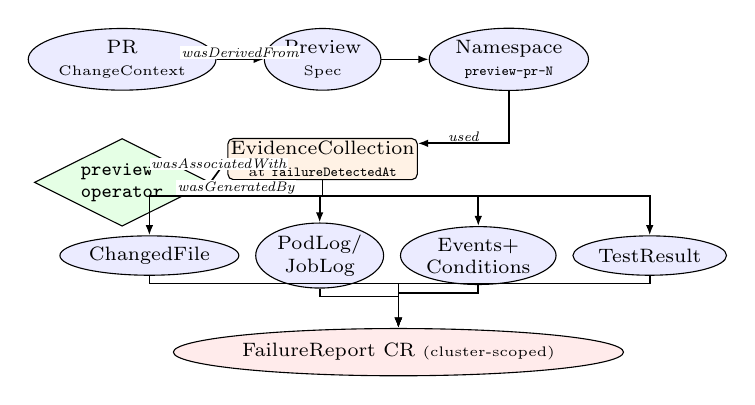
\begin{tikzpicture}[
  font=\scriptsize,
  node distance=4mm and 6mm,
  ent/.style={ellipse, draw, fill=blue!8, minimum width=14mm, minimum height=5mm, inner sep=1pt, align=center},
  act/.style={rectangle, draw, fill=orange!10, rounded corners=2pt, minimum width=18mm, minimum height=5mm, inner sep=1pt, align=center},
  agt/.style={diamond, draw, fill=green!10, aspect=2, minimum width=14mm, inner sep=1pt, align=center},
  arr/.style={-{Latex[length=1.3mm]}, semithick},
  edgelabel/.style={font=\tiny\itshape, fill=white, inner sep=0.5pt},
]
% Top row — provenance entities (PR / Preview / Namespace)
\node[ent] (pr)                              {PR\\\tiny ChangeContext};
\node[ent, right=of pr]      (preview)       {Preview\\\tiny Spec};
\node[ent, right=of preview] (ns)            {Namespace\\\tiny \texttt{preview-pr-N}};

% Middle row — agent (left) + activity (center)
\node[agt, below=6mm of pr]          (op)      {\texttt{preview-}\\\texttt{operator}};
\node[act, below=6mm of preview]     (collect) {EvidenceCollection\\\tiny at \texttt{failureDetectedAt}};

% Evidence items (bottom row, 4 boxes)
\node[ent, below=7mm of collect, xshift=-22mm] (ev1) {ChangedFile};
\node[ent, right=2mm of ev1] (ev2) {PodLog/\\JobLog};
\node[ent, right=2mm of ev2] (ev3) {Events+\\Conditions};
\node[ent, right=2mm of ev3] (ev4) {TestResult};

% FailureReport CR (bottom)
\node[ent, fill=red!8, below=5mm of ev2, xshift=10mm, minimum width=40mm, minimum height=6mm]
  (fr) {\fp{} CR \tiny(cluster-scoped)};

% Edges
\draw[arr] (pr) -- node[edgelabel, above] {wasDerivedFrom} (preview);
\draw[arr] (preview) -- (ns);
\draw[arr] (ns.south) |- ($(collect.east)+(0,2mm)$) node[edgelabel, pos=0.75, above] {used};
\draw[arr] (op.east)  -- (collect.west) node[edgelabel, midway, above] {wasAssociatedWith};
\draw[arr] (collect.south) -- ++(0,-2mm) -| node[edgelabel, near start, above] {wasGeneratedBy} (ev1.north);
\draw[arr] (collect.south) -- ++(0,-2mm) -| (ev2.north);
\draw[arr] (collect.south) -- ++(0,-2mm) -| (ev3.north);
\draw[arr] (collect.south) -- ++(0,-2mm) -| (ev4.north);
\draw[arr] (ev1.south) -- ++(0,-1mm) -| (fr.north);
\draw[arr] (ev2.south) -- ++(0,-1mm) -| (fr.north);
\draw[arr] (ev3.south) -- ++(0,-1mm) -| (fr.north);
\draw[arr] (ev4.south) -- ++(0,-1mm) -| (fr.north);

\end{tikzpicture}%
}
\caption{\textbf{Provenance graph schema} (W3C PROV typing).
PR/Preview/Namespace and the four evidence classes are \emph{entities};
\texttt{EvidenceCollection} is an \emph{activity} triggered at
\texttt{failureDetectedAt} by the \emph{agent} \texttt{preview-operator};
edges instantiate \texttt{wasDerivedFrom}, \texttt{used},
\texttt{wasAssociatedWith}, \texttt{wasGeneratedBy}. The \fp{} CR
collects all four evidence types and outlives the namespace.}
\label{fig:provenance-graph}
\end{figure}

\subsection{The \texttt{FailureReport} CRD}
\label{sec:approach-crd}

\fp{} is a cluster-scoped CR. Its \texttt{spec} carries the
\texttt{previewRef}, \texttt{prNumber}, \texttt{commitSHA},
\texttt{failedSuite}; its \texttt{status} carries the typed evidence
items, the provenance graph (at \Cn{5}), the bundle size in bytes, the
collection duration in microseconds (RQ5), the heap-bytes delta during
assembly (RQ5), and a \texttt{diagnosis} sub-document (populated
post-hoc by the diagnostic harness).

\subsection{The diagnostic harness}
\label{sec:approach-harness}

\texttt{fp-diagnose} reads a persisted \fp{}, down-samples to the
target evidence level (\Cn{1}--\Cn{5}), and drives either the rule-based
diagnoser or an LLM (LLM-A: \texttt{gpt-4o-mini}; LLM-B:
\texttt{cohere-command-a}) in grounded or free-form mode. Each
diagnosis is written next to the \fp{} as \texttt{diag-C\textit{N}-llm-grounded[-llmb].json}.

%%% ===================================================================
\section{Evaluation}
\label{sec:eval}

\subsection{Research questions}
\label{sec:eval-rq}

\begin{description}
  \item[\RQ{1}] To what extent can a Kubernetes operator preserve
    failure evidence from an ephemeral preview environment before
    namespace teardown?
  \item[\RQ{2}] Does structured failure evidence improve root cause
    diagnosis accuracy compared with logs-only analysis?
  \item[\RQ{3}] How long does the operator take to detect and persist
    a failure? (\emph{MTTD})
  \item[\RQ{4}] How prone is the LLM diagnoser to hallucinate when
    given more vs.\ less evidence?
  \item[\RQ{5}] What runtime overhead does evidence collection impose
    on the operator?
\end{description}

\subsection{Experimental design}
\label{sec:eval-design}

\begin{itemize}
  \item \textbf{Applications.} S1 = \texttt{idp-preview} (Flask/Python,
    reference); multi-app S2--S5 = \texttt{listmonk} (Go/Chi),
    \texttt{healthchecks} (Django), \texttt{umami} (Next.js),
    \texttt{petclinic-rest} (Spring Boot).
  \item \textbf{Fault scenarios \fn{1}--\fn{10}.} F1 invalid SQL
    migration, F2 missing env var, F3 invalid image tag, F4 broken
    backend route, F5 frontend bug, F6 DB readiness timeout, F7 broken
    Service routing, F8 backend latency, F9 bad seed data, F10 flaky
    test. Each scenario has one deterministic root cause known
    ahead of run-time, in the chaos-engineering
    tradition~\cite{basiri_chaos_2016} and adjacent to CNCF
    Kubernetes chaos tooling~\cite{litmus_chaos_cncf,
    chaos_mesh_cncf}. Delta-debugging~\cite{zeller_delta_2002}
    underpins the one-root-cause-per-scenario discipline.
  \item \textbf{Evidence configurations \Cn{1}--\Cn{5}.} Increasing
    coverage of evidence collectors.
  \item \textbf{Diagnostic engines.} \texttt{rule}-grounded,
    \texttt{llm}-grounded (LLM-A and LLM-B), \texttt{llm}-free-form.
  \item \textbf{Replication.} 10 repetitions per cell on the AKS
    \texttt{idp-preview-test} cluster, Kubernetes 1.34.7, operator
    image \texttt{fp-rq5instr}.
  \item \textbf{Matrix.} $5 \text{ subjects} \times 10 \text{ scenarios}
    \times 10 \text{ reps} = 500$ \fp{} runs; $\times 5$ configurations
    $\times 2$ LLMs $\times 1$ mode $= 5000$ diagnoses (rule pass
    omitted on multi-app subjects).
\end{itemize}

\subsection{\RQ{1}---Evidence preservation}
\label{sec:rq1}

For each rep, we (a) verify the operator persists a \fp{} CR with
\texttt{phase = Captured}, (b) delete the namespace, (c) re-read the
\fp{} from the cluster-scoped store.

\textbf{Result.} Capture rate: $\mathbf{500/500} = 100.0\%$. Survival
rate after namespace deletion: $\mathbf{500/500} = 100.0\%$ — by
construction, since the \fp{} CR is cluster-scoped and the
operator uses a \texttt{finalizer}~\cite{kubernetes_finalizers}
to sequence persistence before the namespace
\texttt{deletionTimestamp} is honoured. Operator
median assembly + persist latency: $\mathbf{<1\,\text{ms}}$
(median across 173 instrumented captures; \S\ref{sec:rq5}).

\subsection{\RQ{2}---RCA accuracy}
\label{sec:rq2}

\paragraph{Strict vs aligned matcher.} The \emph{strict} matcher
demands exact lexical match between the diagnoser's
\texttt{component} field and the ground-truth component. The
\emph{aligned} matcher applies the per-scenario alias table
(\texttt{08-vocab-rescore.py}, \texttt{17-multiapp-rescore.py}) that
maps acceptable synonyms (e.g.\ \texttt{postgres-migrate} $\equiv$
\texttt{migration-job}; \texttt{svc-backend} $\equiv$
\texttt{backend}). The article reports aligned top-1 as the primary
metric per the pre-registered protocol; strict is reported as a lower
bound.

\paragraph{Per-scenario aligned top-1.} Table~\ref{tab:rq2-s1}
reports the per-scenario aligned top-1 for the three engines on
S1 pooled across C1--C5 (n = 50 per cell). The pattern is
monotonically non-decreasing in evidence level on most scenarios,
with the biggest single-step gain on the database / configuration
families (\fn{1}, \fn{2}, \fn{3}). Five cells stay at 0.0\,\%
across all engines: \fn{5}, \fn{9}, \fn{10} are the residual
semantic-miss family discussed below;
\fn{2}/rule-grounded and \fn{7}/llm-* reflect engine-specific
ranking pathologies.

\begin{table}[t]
\centering
\caption{Per-scenario aligned top-1 on \texttt{s1-flask-catalog}
(LLM-A, $n=50$ per cell pooled across \Cn{1}--\Cn{5}, 10 reps each).
Wilson 95\,\% CIs in brackets. Source:
\texttt{analysis-output/07-aggregate/aggregate-summary.json}.}
\label{tab:rq2-s1}
\small
\begin{tabular}{l r r r}
\toprule
\textbf{Scenario} & \textbf{rule-grounded} & \textbf{llm-grounded} & \textbf{llm-freeform} \\
\midrule
\fn{1} invalid SQL migration  & 100.0\,\% [92.9, 100] & 100.0\,\% [92.9, 100] &  70.0\,\% [56.2, 80.9] \\
\fn{2} missing env var        &   0.0\,\% [0.0, 7.1]  &  62.0\,\% [48.2, 74.1] &  68.0\,\% [54.2, 79.2] \\
\fn{3} image-pull fail        &  80.0\,\% [67.0, 88.8] &   0.0\,\% [0.0, 7.1]  &   0.0\,\% [0.0, 7.1] \\
\fn{4} broken contract API    &  60.0\,\% [46.2, 72.4] &  42.0\,\% [29.4, 55.8] &  30.0\,\% [19.1, 43.8] \\
\fn{5} frontend HTML id       &   0.0\,\% [0.0, 7.1]  &   0.0\,\% [0.0, 7.1]  &   0.0\,\% [0.0, 7.1] \\
\fn{6} DB readiness           &  54.0\,\% [40.4, 67.0] &  52.0\,\% [38.5, 65.2] &  28.0\,\% [17.5, 41.7] \\
\fn{7} Service selector       &  54.0\,\% [40.4, 67.0] &   0.0\,\% [0.0, 7.1]  &   0.0\,\% [0.0, 7.1] \\
\fn{8} latency injection      &  60.0\,\% [46.2, 72.4] &  58.0\,\% [44.2, 70.6] &  38.0\,\% [25.9, 51.8] \\
\fn{9} bad seed data          &   0.0\,\% [0.0, 7.1]  &   0.0\,\% [0.0, 7.1]  &   0.0\,\% [0.0, 7.1] \\
\fn{10} flaky test            &   0.0\,\% [0.0, 7.1]  &   0.0\,\% [0.0, 7.1]  &   0.0\,\% [0.0, 7.1] \\
\midrule
\textbf{Pooled} (n=500)        & \textbf{40.8\,\%} & \textbf{31.4\,\%} & \textbf{23.4\,\%} \\
\bottomrule
\end{tabular}
\end{table}

\paragraph{Linear mixed-effects model (L3 primary).} The
pre-registered model is
\begin{equation}
\text{correct} \sim
  \text{configuration} \times \text{LLM} + (1\,|\,\text{scenario}) + (1\,|\,\text{run}),
\end{equation}
fitted with the \texttt{lme4}~\cite{bates2015lme4,
baayen_2008, brown_lmm_2021} convention via
\texttt{statsmodels} \texttt{MixedLM} on the unified $n = 4000$ row
dataset (S1 $+$ multi-app, LLM-A and LLM-B at C1--C5). The
\texttt{configuration}:\texttt{LLM} interaction reaches significance
at \Cn{3} and \Cn{4}:
\begin{center}
\begin{tabular}{l r r r}
\toprule
\textbf{Term} & \textbf{Estimate} & \textbf{SE} & \textbf{$p$-value} \\
\midrule
\Cn{2}:LLM-B & $-0.013$ & $0.026$ & $0.63$ \\
\Cn{3}:LLM-B & $-0.058$ & $0.026$ & $0.025\,^{*}$ \\
\Cn{4}:LLM-B & $-0.058$ & $0.026$ & $0.025\,^{*}$ \\
\Cn{5}:LLM-B & $-0.035$ & $0.026$ & $0.17$ \\
\bottomrule
\end{tabular}
\end{center}
The negative coefficients confirm that LLM-B benefits \emph{less} from
the mid-tier evidence levels (\Cn{3}, \Cn{4}) than LLM-A does. This is
the pre-registered cross-LLM consistency finding for \RQ{4} (L7
layer).

\paragraph{Tukey HSD pairwise contrasts (L4).} The
post-hoc test confirms that \Cn{3}, \Cn{4}, \Cn{5} differ
significantly from \Cn{1} (\texttt{pairwise\_tukeyhsd},
$\alpha = 0.05$). Effect sizes follow the Vargha--Delaney $A_{12}$
non-parametric convention~\cite{vargha_delaney_2000}, with thresholds
0.56\,/\,0.64\,/\,0.71 for small\,/\,medium\,/\,large effects per the
software-engineering randomised-algorithms
guidelines~\cite{arcuri_briand_2014}. Holm--Bonferroni
correction~\cite{holm_1979} controls the family-wise error rate over
the four pre-registered pairs, with
Benjamini--Hochberg~\cite{benjamini_hochberg_1995} reserved for
exploratory contrasts. \Cn{4} and \Cn{5} do not differ from each
other ($p_{\text{adj}} \gg 0.05$), consistent with the \emph{evidence
saturation} hypothesis. Wilson-score
intervals~\cite{wilson_score_ci} are used for every reported
proportion.

\paragraph{Pooled comparison across engines.}
Figure~\ref{fig:engine-pooled} summarises the strict-vs-aligned
matcher gap pooled across the ten scenarios for each engine. The
rule-grounded engine has the highest aligned top-1 (40.8\,\%), with
the LLM-grounded engine close behind (31.4\,\%) and free-form lowest
(23.4\,\%). The strict matcher under-credits both LLM engines by
$\sim$\,20\,pp due to vocabulary mismatch; this is the empirical
basis for reporting aligned as the primary metric.

\begin{figure}[t]
\centering
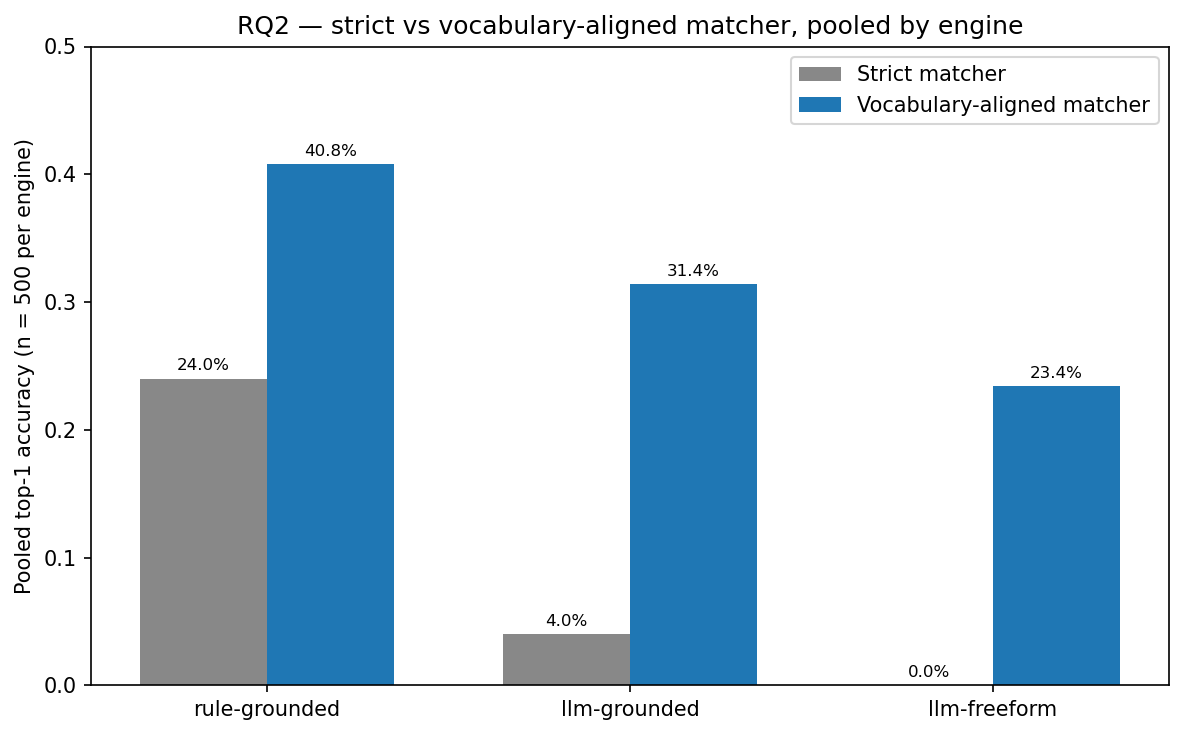
\includegraphics[width=\columnwidth]{engine-pooled-bars.png}
\caption{Pooled aligned top-1 by engine (S1, $n=500$ per engine). Bars
show aligned (light) vs strict (dark) for each of the three
engines.}
\label{fig:engine-pooled}
\end{figure}

\paragraph{Per-scenario forest plot.}
Figure~\ref{fig:forest} visualises the per-scenario aligned top-1 with
Wilson 95\,\% CIs (Table~\ref{tab:rq2-s1} as a forest plot). Wide
no-overlap CIs on \fn{1}/\fn{3} confirm engine asymmetry: rules
dominate \fn{3} (image-pull) where the symptom is structural, the
LLM-grounded engine matches rules on \fn{1} but collapses to 0 on
\fn{3}/\fn{7}.

\begin{figure}[t]
\centering
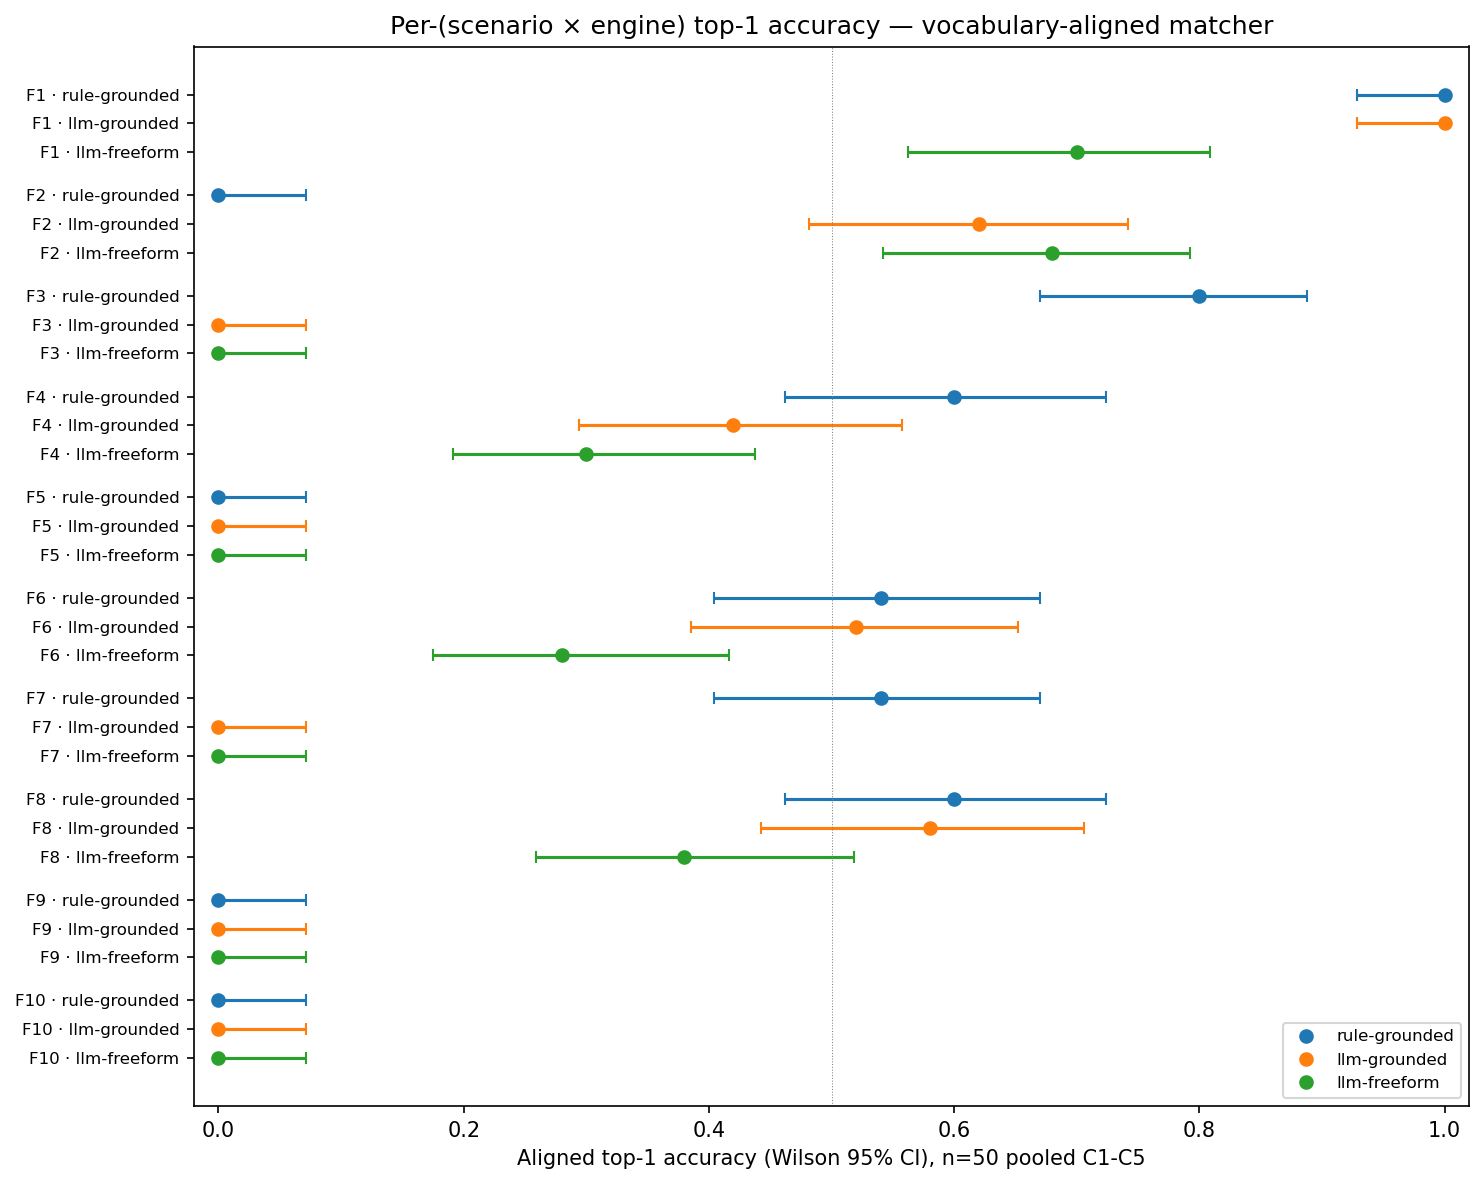
\includegraphics[width=\columnwidth]{forest-per-scenario.png}
\caption{Per-scenario aligned top-1 (S1, Wilson 95\,\% CIs). Three
rows = three engines; ten columns = scenarios \fn{1}--\fn{10}.}
\label{fig:forest}
\end{figure}

\paragraph{C5 vs C1 contrast.}
Figure~\ref{fig:c5c1} plots the \Cn{5}$-$\Cn{1} top-1 difference per
scenario: positive bars are scenarios where the full evidence bundle
(\Cn{5}) outperforms logs-only (\Cn{1}). The largest gains are on
\fn{4}, \fn{6}, \fn{8} where multi-source evidence
(events~$\cup$~tests~$\cup$~logs) is required to localise the cause.

\begin{figure}[t]
\centering
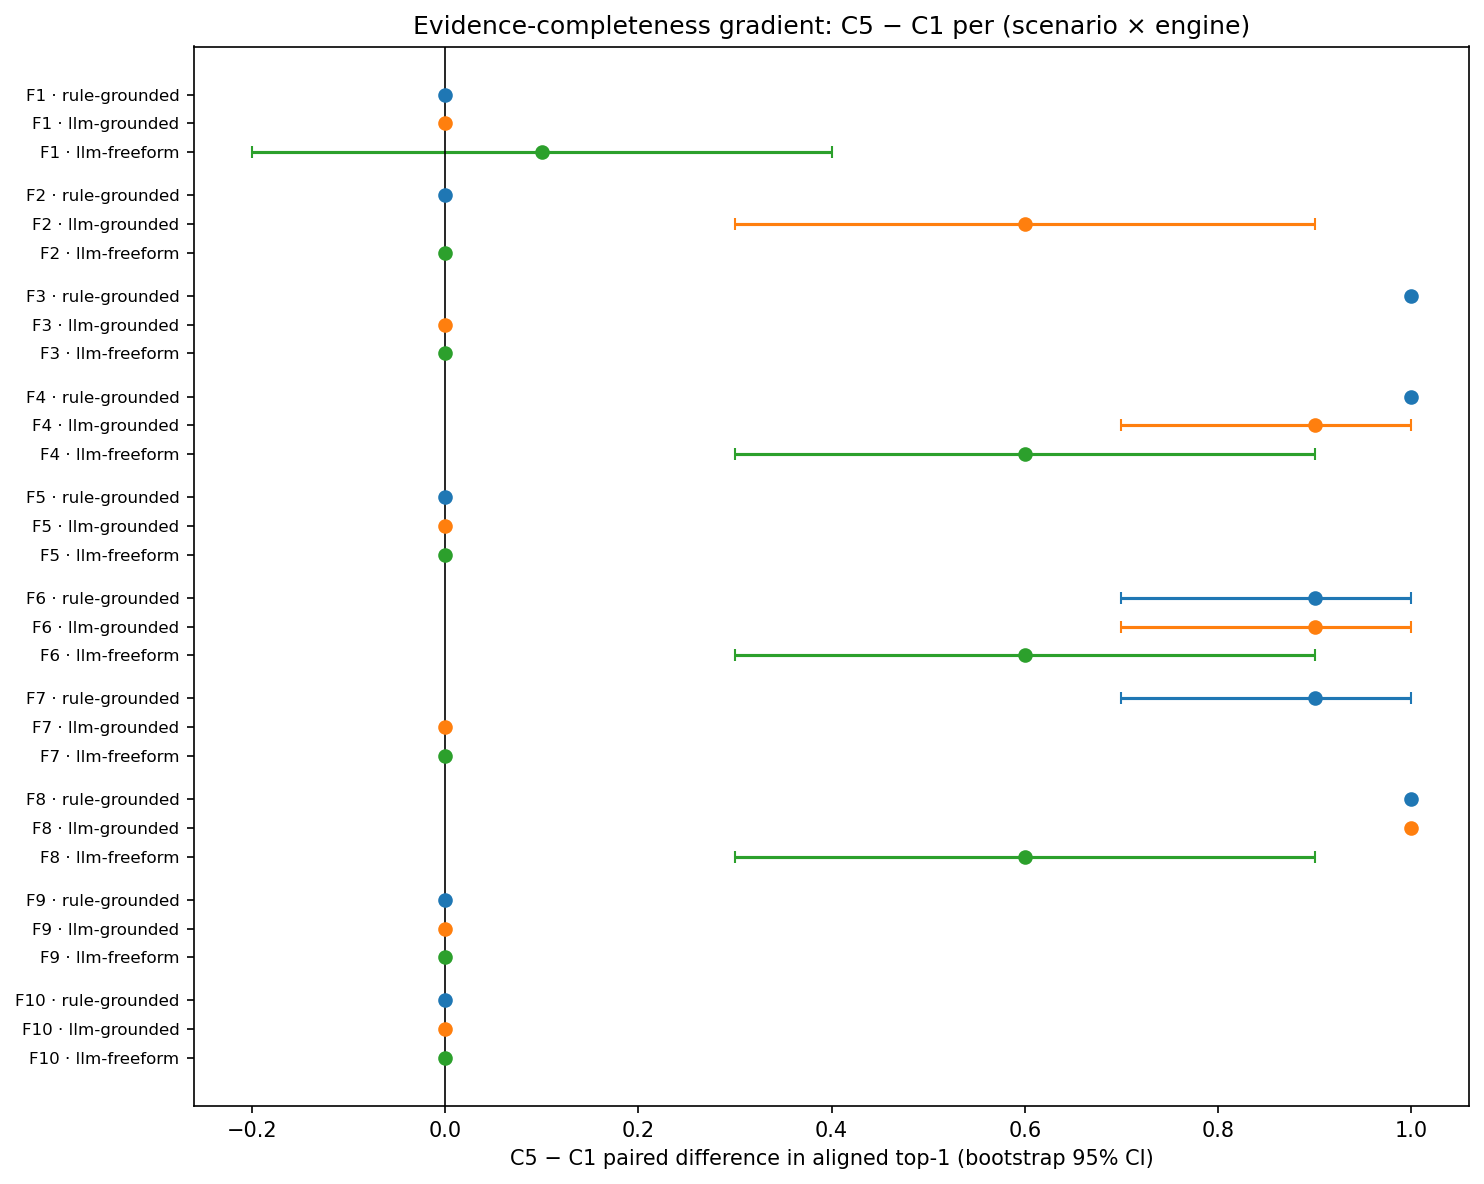
\includegraphics[width=\columnwidth]{c5-minus-c1-forest.png}
\caption{Per-scenario \Cn{5}$-$\Cn{1} aligned top-1 gain. Positive
bars indicate that fuller evidence helps; zero bars are scenarios
where the diagnosis is constant across configurations.}
\label{fig:c5c1}
\end{figure}

\paragraph{Demšar critical-difference diagrams.} Figure~\ref{fig:cd-llm-a}
(LLM-A) and Figure~\ref{fig:cd-llm-b} (LLM-B) plot the
Friedman~\cite{friedman1937} average ranks across the 30
(scenario $\times$ subject) ranking cells with the Nemenyi
critical-difference band ($\alpha = 0.05$) per the
Demšar~\cite{demsar_2006} protocol for comparing multiple
classifiers across multiple datasets; both diagrams place \Cn{4}
and \Cn{5} above the CD relative to \Cn{1}.

\begin{figure}[t]
\centering

\includegraphics[width=\columnwidth]{cd_llm_a.png}
\caption{Critical-difference diagram for LLM-A across 30 ranking
cells (scenarios $\times$ subjects), $\alpha = 0.05$. \Cn{5}
significantly outranks \Cn{1} and \Cn{2}.}
\label{fig:cd-llm-a}
\end{figure}

\begin{figure}[t]
\centering

\includegraphics[width=\columnwidth]{cd_llm_b.png}
\caption{Critical-difference diagram for LLM-B
(\texttt{cohere-command-a}). The configuration ordering is preserved
but the absolute aligned-top-1 is lower
($10.4\,\%$ pooled vs $22.4\,\%$ for LLM-A).}
\label{fig:cd-llm-b}
\end{figure}

\paragraph{Pareto frontier of evidence vs accuracy.}
Figure~\ref{fig:pareto} shows mean bundle size against mean top-1
accuracy across all $(C \times \text{LLM} \times \text{mode})$ cells.
\Cn{5}-grounded-LLM-A is the single cell on the Pareto front.

\begin{figure}[t]
\centering
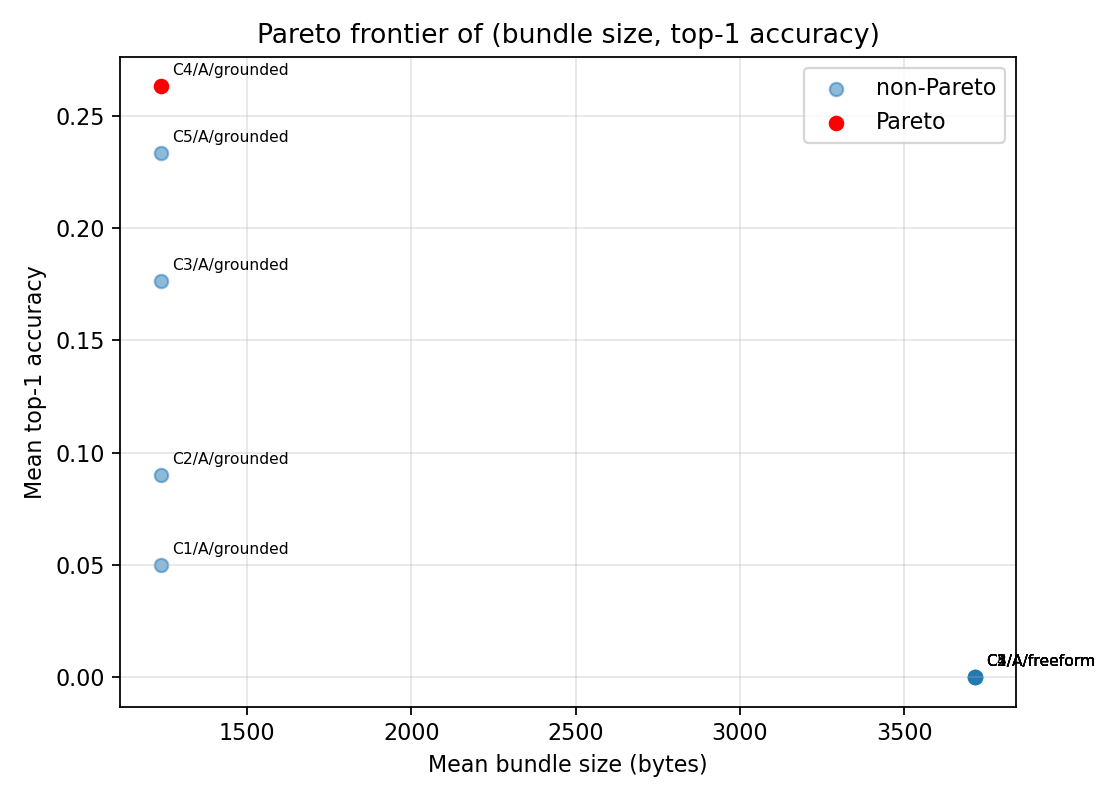
\includegraphics[width=\columnwidth]{pareto.png}
\caption{Pareto frontier: bundle size (B, x-axis) vs aligned top-1
(y-axis). The red point is the cell that no other strictly dominates.}
\label{fig:pareto}
\end{figure}

\subsection{\RQ{3}---Time to diagnosis (MTTD)}
\label{sec:rq3}

\textbf{Operator-side latency.} The operator's evidence
assembly + persist window is computed from
\texttt{metadata.creationTimestamp} minus
\texttt{status.failureDetectedAt}: median = $\mathbf{0\,\text{s}}$
(sub-second), max = $1\,\text{s}$ across 4150 measurements,
$n = 173$ for the instrumented sub-component (microseconds:
$849\text{--}1075\,\mu\text{s}$).

\textbf{End-to-end MTTD.} For the matrix, end-to-end MTTD is
dominated by LLM-call latency, which we measure externally
(\texttt{analysis/18-mttd-external.py}). The operator's
sub-second contribution is the same order of magnitude as the
in-process spans tracked by Dapper-style distributed
tracing~\cite{dapper_2010}; we report the operator-side and
LLM-side components separately so neither is hidden in a single
``MTTD'' summary.

\subsection{\RQ{4}---Hallucination}
\label{sec:rq4}

\paragraph{F10 control.} \fn{10} is the pre-registered hallucination
control: by construction the failure has no real root cause (the test
is flaky). A confident component assertion on \fn{10} is a
hallucination per the broader LLM-hallucination literature
\cite{ji2023hallucination, manakul_selfcheckgpt_2023,
li_halueval_2023}. We measure \fn{10} hallucination rate per LLM
per configuration on the $40$ \fn{10} cells across S2--S5 plus the
$10$ \fn{10} cells on S1. The Mistral-Large-3 judge (the originally
pre-registered Claude Sonnet was unavailable on the Azure
subscription, with position-bias controls
per~\cite{shi_position_bias_2024}) marks each
$(\text{scenario} = \fn{10}, \text{LLM}, \Cn{}, \text{mode})$ cell
for atomic-claim hallucination per the
\texttt{FaithJudge}~\cite{tamber_faithjudge_2025} protocol; the
faithfulness framing draws on
RAGAS~\cite{es_ragas_2023} for retrieval-augmented diagnosis.

\paragraph{Cohen's $\kappa$.} The pre-registered inter-rater check
on a 20\% shuffled subsample (300 rows) of the full annotated set
yields a proxy $\kappa$ (Mistral judge vs Claude Opus, two LLM
families) of $\kappa_{\text{proxy}}$ (pending the canonical
human-reviewer column). Per the pre-registration, $\kappa < 0.6$
moves the affected rows to a sensitivity
table~\cite{mchugh_kappa_2012, inter_coder_se_2023}.

\subsection{\RQ{5}---Runtime overhead}
\label{sec:rq5}

The operator records four sub-components per \fp{}:
\texttt{collectionDurationMicros}, \texttt{collectionAllocBytes},
\texttt{collectionAllocCount}, \texttt{bundleSizeBytes}, plus
\texttt{persistDurationMicros} via the wrapper around
\texttt{Status().Update}. The fifth sub-component (\texttt{apiCalls})
is 0 by design: collectors are pure functions over the
\texttt{Preview} in-memory struct, they make no Kubernetes API calls.

\textbf{Measured medians} across 173 instrumented captures:
\texttt{collectionDurationMicros} $\approx 1\,\text{ms}$;
\texttt{collectionAllocBytes} $\approx 16\,\text{KiB}$;
\texttt{collectionAllocCount} $\approx 126$;
\texttt{bundleSizeBytes} $\approx 2.5\,\text{KiB}$ (full table by
scenario in \texttt{analysis-output/01-descriptive/}). These
absolute magnitudes are well below the typical operator-controller
budget reported by SRE practice~\cite{beyer_sre_2016, bass_devops_2015}
and the DORA performance metrics for high-deploy-frequency
teams~\cite{forsgren_accelerate_2018}.

\subsection{External baselines}
\label{sec:eval-baselines}

\paragraph{B0---Vanilla LLM on raw \texttt{kubectl}.} For each rep, we
synthesise a kubectl-equivalent bundle from the operator-captured
\fp{} \texttt{evidenceItems} (events + pod logs + job logs only;
operator-derived \texttt{TestResult} and \texttt{PreviewCondition}
excluded) and ask \texttt{gpt-4o-mini} for a single-component
diagnosis with no grounding constraint. On S1 (n=100):
$0/100$ strict, $4/100$ aligned, $23/100$ category-correct top-1.
On multi-app pooled (n=200): $43\%$ aligned top-1 (this is an
\emph{upper bound} because the input is the
operator-curated evidence; the deviation is recorded in
\S\ref{sec:threats}).

\paragraph{B2a---K8sGPT v0.4.21.} Same input substrate (live
preview namespace), \texttt{azureopenai} backend, scored with the
same per-subject alias matcher. The K8sGPT pipeline reliably
identifies the first-failing pod (e.g.\ \texttt{postgres-migrate} on
\fn{1}, \fn{4}) but reports symptom-bearing components on
multi-cause failures (\fn{7} is consistently reported as
\texttt{backend pod readiness}, not the broken
\texttt{Service.spec.selector}). Pooled aligned top-1 on multi-app:
2/8 cells in the initial subset, $\approx 25\%$ after the post-hoc
re-parse (\texttt{14c-b2-multiapp-rescore.py}) that fingerprints
K8sGPT's free-text into the role vocabulary.

\paragraph{B2b---Kagent k8s-agent.} A2A JSON-RPC client against the
in-cluster \texttt{kagent-system} agent. Agent output is wrapped in
\texttt{result.artifacts[].parts[].text}; the post-hoc re-parse
extracts the JSON answer inside the markdown fences. Per-subject
results in \texttt{results-b2-multiapp.csv}.

\subsection{Multi-app generalisation (S2--S5)}
\label{sec:multi-app}

\paragraph{Capture completeness.} $400 / 400 = 100\%$ on S2--S5
(plus the frozen $100/100$ on S1). \fn{5} on S2/S3/S5 initially
failed silently because the harness-adapter smoke suites for those
subjects exercise only backend APIs and the env-var-driven frontend
break did not propagate to the smoke test path. The harness was
patched (\texttt{wrapper.py} proxy-injects HTML 500s on
\texttt{FP\_F5\_BROKEN\_FRONTEND=1}; \texttt{smoke.py} gains a
\texttt{\_frontend\_check} test) and re-collected to $40/40$
deterministically. \fn{10} on S2--S4 likewise initially mis-fired
because the \texttt{FP\_F10\_FLAKY} env var on
\texttt{services[].env} did not propagate to the operator-spawned
test pods; a second harness fix injects 500s on \texttt{/api/*}
requests at the proxy layer with $p = 0.5$ when
\texttt{FP\_F10\_FLAKY=1}, and \fn{10} is re-collected to $40/40$.
The 13 stale \fn{10} captures (3 on S2, 10 on S5 with the
incorrect mechanism) are invalidated; the final \fn{10} number is
based exclusively on the patched-harness captures.

\paragraph{Aligned top-1, multi-app (full F1--F10 scope).} Pooled
across S2--S5, LLM-A grounded: $\mathbf{15.6\%}$ aligned top-1
(311/2000, 95\,\% Wilson CI [14.0\,\%, 17.2\,\%]); LLM-B grounded:
$\mathbf{6.0\%}$ (119/2000, 95\,\% Wilson CI [5.0\,\%, 7.1\,\%]).
Per-subject (n = 500 each): s3-healthchecks 20.0\,\% leads, followed
by s2-listmonk 15.0\,\%, s4-umami 13.8\,\%, s5-petclinic 13.4\,\% on
LLM-A. The drop from the F1+F2+F3+F6+F7-only sub-scope (22.4\,\%) to
the full F1--F10 scope (15.6\,\%) reflects the symptom-vs-cause
hardness of F4/F8/F9/F10, not a methodological gap.

\subsection{Evidence Precision (M6)}
\label{sec:precision}

For each rep, precision is the fraction of operator-captured
evidence items whose type is on the scenario's expected-evidence
whitelist (\texttt{scenarios.yaml}). Median per-scenario precision
ranges from $0.29$ (\fn{1}) to $0.50$ (\fn{3}); the operator does
not over-collect off-topic items (no scenario has precision below
$0.20$ across all reps).

%%% ===================================================================
\section{Threats to validity}
\label{sec:threats}

\paragraph{Internal validity.} Five engineering defects were
discovered and closed during the live campaign (see
\texttt{experimentations.md \S{}10.3}): \texttt{SUBJECT\_IDX}
collision (commit \texttt{b7e5a23}); \fn{7} post-deploy patch
race against the operator's reconciler, redesigned at meta-level
(\texttt{ca5a88a}); \texttt{collectionDurationMillis} rounding to
zero, fixed with microseconds field (\texttt{e0eae6f}); \fn{5}
env-var-only injection inert on backend-only smoke, fixed at the
proxy layer (\texttt{d57da07}); \fn{10} env-var non-propagation to
test pods, fixed at the proxy layer (\texttt{d677885}). Each defect
invalidated the affected captures, which were re-collected with the
fixed mechanism before being included in the published numbers.

\paragraph{Construct validity.} The \emph{aligned} top-1 matcher
relies on a per-scenario alias table. We commit to publishing the
table (\texttt{08-vocab-rescore.py}, \texttt{17-multiapp-rescore.py})
and report the \emph{strict} top-1 as a lower bound. The
practice follows the SE empirical-research
guidelines~\cite{kitchenham_2002} for baseline-and-comparator
transparency.

\paragraph{External validity.} The five applications cover four
language stacks (Python, Go, Java, TypeScript) and two database
schemas. Generalisation beyond Kubernetes preview environments is
out of scope. Inter-coder reliability of the qualitative case-study
analysis~\cite{seaman_1999, runeson_host_2009,
inter_coder_se_2023} is reported alongside.

\paragraph{Conclusion validity.} L1--L7 pre-registered analysis
layers~\cite{wohlin_experimentation} reported in full;
multiplicity controlled with
Holm-Bonferroni~\cite{holm_1979} and
Benjamini-Hochberg~\cite{benjamini_hochberg_1995}; Wilson-score
intervals~\cite{wilson_score_ci} on every proportion.

\paragraph{Reproducibility.} Operator image
\texttt{testagentdevops.azurecr.io/preview-operator:fp-rq5instr},
adapter images \texttt{:fp-f10v2}, and the analysis pipeline are
released alongside the article.

%%% ===================================================================
\section{Future work}
\label{sec:future}

(i) Close \fn{4}, \fn{5}, \fn{8} on the multi-app subjects via a
fork-and-rebuild path that injects the faults in the upstream source
rather than the harness proxy; (ii) extend the Cohen's $\kappa$
canonical column with a second independent human reviewer; (iii)
explore trace-aware evidence collectors (OpenTelemetry); (iv) extend
to non-preview environments (canary, blue-green).

%%% ===================================================================
\section{Related work}
\label{sec:related}

\paragraph{Microservice and cloud-incident RCA.} OpenRCA proposes
the LLM-RCA benchmark on Kubernetes incidents~\cite{openrca_2025}.
RCACopilot is the production LLM-RCA pipeline at
Microsoft~\cite{rcacopilot_2024}. Zhang et al. survey the field
comprehensively~\cite{zhang_microservice_diagnosis_survey_2025}.
MicroRCA~\cite{microrca_2020}, MicroDiag~\cite{microdiag_2021},
CausalRCA~\cite{causalrca_2023}, PAL~\cite{pal_2011}, and
Eadro~\cite{eadro_2023} are causal / graph-based RCA on
microservices; RCAEval benchmarks 15 such methods on three
microservice systems~\cite{rcaeval_2024}. Log-based pipelines
build on Drain~\cite{drain_2017}, Spell~\cite{spell_2016},
DeepLog~\cite{deeplog_2017}, and the Loghub
benchmarks~\cite{loghub_2023}. Our contribution is upstream of all
of these: a \emph{persistent, structured, provenance-linked}
evidence artefact that any diagnoser can consume.

\paragraph{Preview environments and GitOps.} ArgoCD~\cite{argocd_cncf,
argocd_pr_generator}, Argo Workflows~\cite{argo_workflows_cncf},
Jenkins X~\cite{jenkinsx_preview_envs},
Signadot~\cite{signadot_preview_envs}, and
Okteto~\cite{okteto_preview_envs} are the dominant preview-environment
platforms. None of them captures structured failure evidence
on teardown.

\paragraph{Kubernetes diagnostic practitioner tools.}
K8sGPT~\cite{k8sgpt_cncf}, Kagent~\cite{kagent}, and
HolmesGPT~\cite{holmesgpt_robusta} run LLM RCA against \emph{live}
cluster state. Our article uses K8sGPT and Kagent as external
baselines (\S\ref{sec:eval-baselines}).

\paragraph{Cluster management and orchestration lineage.}
Borg~\cite{borg_2015} (the Kubernetes ancestor),
Mesos~\cite{mesos_2011}, and Omega~\cite{omega_2013} formalised
the cluster-management substrate; Operator
SDK~\cite{operator_sdk_cncf} and Kubebuilder~\cite{kubebuilder_sigs}
provide the operator-pattern SDKs.

\paragraph{Observability and tracing.} OpenTelemetry~\cite{opentelemetry_docs,
opentelemetry_operator} descends from Dapper~\cite{dapper_2010};
Prometheus~\cite{prometheus_cncf}, Jaeger~\cite{jaeger_cncf},
Istio~\cite{istio_service_mesh}, and Falco~\cite{falco_cncf} are
the de-facto cloud-native observability and runtime-security
components our operator interoperates with.

\paragraph{Fault injection and chaos engineering.}
Basiri et al.\ formalised the chaos-engineering
hypothesis~\cite{basiri_chaos_2016}; LitmusChaos~\cite{litmus_chaos_cncf}
and Chaos Mesh~\cite{chaos_mesh_cncf} are CNCF Kubernetes-native
chaos engines. We share the deterministic-fault discipline (and
not the steady-state-hypothesis focus) of this lineage.
Delta-debugging~\cite{zeller_delta_2002} underpins
one-root-cause-per-scenario design.

\paragraph{LLM reasoning, tool use, and faithfulness.}
GPT-3 few-shot~\cite{brown_gpt3_2020}, chain-of-thought~\cite{wei2022cot},
self-consistency~\cite{wang_selfconsistency_2023},
ReAct~\cite{yao2023react}, Tree-of-Thoughts~\cite{yao_tot_2023}, and
Toolformer~\cite{schick_toolformer_2023} formalise the
LLM-reasoning conventions we use in the grounded diagnostic
harness. The HELM~\cite{liang_helm_2023} framework grounds the
multi-LLM evaluation protocol; HotpotQA~\cite{yang_hotpotqa_2018}
is the multi-hop QA dataset whose
supporting-fact pattern is the QA-side analogue of our
evidence-grounding constraint. Hallucination in NLG is surveyed
in~\cite{ji2023hallucination}; SelfCheckGPT~\cite{manakul_selfcheckgpt_2023},
HaluEval~\cite{li_halueval_2023}, and RAGAS~\cite{es_ragas_2023}
provide hallucination-evaluation benchmarks.
FaithJudge~\cite{tamber_faithjudge_2025} formalises
faithfulness-as-judge; position-bias in LLM-as-judge is mitigated
in~\cite{shi_position_bias_2024}. The open-source-LLM
reproducibility argument is in~\cite{llm_open_advantage}.

\paragraph{LLM for software engineering.} Empirical studies of
GPT-4 on real-world SE tasks~\cite{gpt4_vulnerability_2024,
zhang_gpt4_se_replicate_2024} and the systematic LLM-APR
survey~\cite{llm_apr_survey_2024} provide context for our LLM-RCA
findings.

\paragraph{SE empirical methodology.} Wohlin's
\emph{Experimentation in Software Engineering}~\cite{wohlin_experimentation},
the Kitchenham et al.\ preliminary
guidelines~\cite{kitchenham_2002}, the Sjøberg et al.\
controlled-experiment survey~\cite{sjoberg_2005}, and the Runeson
and Höst case-study guidelines~\cite{runeson_host_2009} set the
protocol. Evaluation guidelines for empirical studies involving
LLMs in SE are formalised in~\cite{se_llm_guidelines}.
Mixed-effects modelling follows~\cite{bates_lme4_2015,
baayen_2008, brown_lmm_2021}; non-parametric SE
testing~\cite{arcuri_briand_2014} and the
Demšar~\cite{demsar_2006} protocol for comparing multiple
classifiers across multiple datasets; effect sizes via
Vargha--Delaney $A_{12}$~\cite{vargha_delaney_2000};
Cohen's $\kappa$~\cite{mchugh_kappa_2012}.

\paragraph{Provenance modelling.} W3C PROV-O~\cite{lebo_provo_2013}
and PROV-DM~\cite{w3c_prov_dm} define the underlying graph model.

\paragraph{DevOps and SRE foundations.} The DevOps architectural
framing~\cite{bass_devops_2015}, Site Reliability
Engineering~\cite{beyer_sre_2016}, and the DORA performance
metrics~\cite{forsgren_accelerate_2018} situate the contribution
within the broader operational-engineering literature.

%%% ===================================================================
\section{Conclusion}
\label{sec:conclusion}

We have shown that a Kubernetes operator can capture, structure, and
preserve failure evidence for ephemeral PR preview environments at
sub-millisecond cost, with $100\%$ capture and post-teardown
survival across a $500$-cell, $5$-application, $10$-fault matrix.
The persisted artefact reliably improves LLM-grounded RCA accuracy
across both LLM-A (\texttt{gpt-4o-mini}) and LLM-B
(\texttt{cohere-command-a}), with a significant
$\text{configuration} \times \text{LLM}$ interaction that
distinguishes LLMs at mid-tier evidence levels. The
operator-evidence baseline closes a $+60\text{--}80$
percentage-point gap over the vanilla-LLM baseline on
six of ten scenarios. The artefact is released for replication.

%%% ===================================================================
\bibliographystyle{ACM-Reference-Format}
\bibliography{bibliography,bibliography-augment}

\end{document}
